% Options for packages loaded elsewhere
\PassOptionsToPackage{unicode}{hyperref}
\PassOptionsToPackage{hyphens}{url}
%
\documentclass[
  ignorenonframetext,
]{beamer}
\usepackage{pgfpages}
\setbeamertemplate{caption}[numbered]
\setbeamertemplate{caption label separator}{: }
\setbeamercolor{caption name}{fg=normal text.fg}
\beamertemplatenavigationsymbolsempty
% Prevent slide breaks in the middle of a paragraph
\widowpenalties 1 10000
\raggedbottom
\setbeamertemplate{part page}{
  \centering
  \begin{beamercolorbox}[sep=16pt,center]{part title}
    \usebeamerfont{part title}\insertpart\par
  \end{beamercolorbox}
}
\setbeamertemplate{section page}{
  \centering
  \begin{beamercolorbox}[sep=12pt,center]{part title}
    \usebeamerfont{section title}\insertsection\par
  \end{beamercolorbox}
}
\setbeamertemplate{subsection page}{
  \centering
  \begin{beamercolorbox}[sep=8pt,center]{part title}
    \usebeamerfont{subsection title}\insertsubsection\par
  \end{beamercolorbox}
}
\AtBeginPart{
  \frame{\partpage}
}
\AtBeginSection{
  \ifbibliography
  \else
    \frame{\sectionpage}
  \fi
}
\AtBeginSubsection{
  \frame{\subsectionpage}
}
\usepackage{amsmath,amssymb}
\usepackage{lmodern}
\usepackage{iftex}
\ifPDFTeX
  \usepackage[T1]{fontenc}
  \usepackage[utf8]{inputenc}
  \usepackage{textcomp} % provide euro and other symbols
\else % if luatex or xetex
  \usepackage{unicode-math}
  \defaultfontfeatures{Scale=MatchLowercase}
  \defaultfontfeatures[\rmfamily]{Ligatures=TeX,Scale=1}
\fi
% Use upquote if available, for straight quotes in verbatim environments
\IfFileExists{upquote.sty}{\usepackage{upquote}}{}
\IfFileExists{microtype.sty}{% use microtype if available
  \usepackage[]{microtype}
  \UseMicrotypeSet[protrusion]{basicmath} % disable protrusion for tt fonts
}{}
\makeatletter
\@ifundefined{KOMAClassName}{% if non-KOMA class
  \IfFileExists{parskip.sty}{%
    \usepackage{parskip}
  }{% else
    \setlength{\parindent}{0pt}
    \setlength{\parskip}{6pt plus 2pt minus 1pt}}
}{% if KOMA class
  \KOMAoptions{parskip=half}}
\makeatother
\usepackage{xcolor}
\IfFileExists{xurl.sty}{\usepackage{xurl}}{} % add URL line breaks if available
\IfFileExists{bookmark.sty}{\usepackage{bookmark}}{\usepackage{hyperref}}
\hypersetup{
  pdftitle={R Workshop / Duke MEM},
  pdfauthor={Zahid Asghar},
  hidelinks,
  pdfcreator={LaTeX via pandoc}}
\urlstyle{same} % disable monospaced font for URLs
\newif\ifbibliography
\usepackage{color}
\usepackage{fancyvrb}
\newcommand{\VerbBar}{|}
\newcommand{\VERB}{\Verb[commandchars=\\\{\}]}
\DefineVerbatimEnvironment{Highlighting}{Verbatim}{commandchars=\\\{\}}
% Add ',fontsize=\small' for more characters per line
\usepackage{framed}
\definecolor{shadecolor}{RGB}{248,248,248}
\newenvironment{Shaded}{\begin{snugshade}}{\end{snugshade}}
\newcommand{\AlertTok}[1]{\textcolor[rgb]{0.94,0.16,0.16}{#1}}
\newcommand{\AnnotationTok}[1]{\textcolor[rgb]{0.56,0.35,0.01}{\textbf{\textit{#1}}}}
\newcommand{\AttributeTok}[1]{\textcolor[rgb]{0.77,0.63,0.00}{#1}}
\newcommand{\BaseNTok}[1]{\textcolor[rgb]{0.00,0.00,0.81}{#1}}
\newcommand{\BuiltInTok}[1]{#1}
\newcommand{\CharTok}[1]{\textcolor[rgb]{0.31,0.60,0.02}{#1}}
\newcommand{\CommentTok}[1]{\textcolor[rgb]{0.56,0.35,0.01}{\textit{#1}}}
\newcommand{\CommentVarTok}[1]{\textcolor[rgb]{0.56,0.35,0.01}{\textbf{\textit{#1}}}}
\newcommand{\ConstantTok}[1]{\textcolor[rgb]{0.00,0.00,0.00}{#1}}
\newcommand{\ControlFlowTok}[1]{\textcolor[rgb]{0.13,0.29,0.53}{\textbf{#1}}}
\newcommand{\DataTypeTok}[1]{\textcolor[rgb]{0.13,0.29,0.53}{#1}}
\newcommand{\DecValTok}[1]{\textcolor[rgb]{0.00,0.00,0.81}{#1}}
\newcommand{\DocumentationTok}[1]{\textcolor[rgb]{0.56,0.35,0.01}{\textbf{\textit{#1}}}}
\newcommand{\ErrorTok}[1]{\textcolor[rgb]{0.64,0.00,0.00}{\textbf{#1}}}
\newcommand{\ExtensionTok}[1]{#1}
\newcommand{\FloatTok}[1]{\textcolor[rgb]{0.00,0.00,0.81}{#1}}
\newcommand{\FunctionTok}[1]{\textcolor[rgb]{0.00,0.00,0.00}{#1}}
\newcommand{\ImportTok}[1]{#1}
\newcommand{\InformationTok}[1]{\textcolor[rgb]{0.56,0.35,0.01}{\textbf{\textit{#1}}}}
\newcommand{\KeywordTok}[1]{\textcolor[rgb]{0.13,0.29,0.53}{\textbf{#1}}}
\newcommand{\NormalTok}[1]{#1}
\newcommand{\OperatorTok}[1]{\textcolor[rgb]{0.81,0.36,0.00}{\textbf{#1}}}
\newcommand{\OtherTok}[1]{\textcolor[rgb]{0.56,0.35,0.01}{#1}}
\newcommand{\PreprocessorTok}[1]{\textcolor[rgb]{0.56,0.35,0.01}{\textit{#1}}}
\newcommand{\RegionMarkerTok}[1]{#1}
\newcommand{\SpecialCharTok}[1]{\textcolor[rgb]{0.00,0.00,0.00}{#1}}
\newcommand{\SpecialStringTok}[1]{\textcolor[rgb]{0.31,0.60,0.02}{#1}}
\newcommand{\StringTok}[1]{\textcolor[rgb]{0.31,0.60,0.02}{#1}}
\newcommand{\VariableTok}[1]{\textcolor[rgb]{0.00,0.00,0.00}{#1}}
\newcommand{\VerbatimStringTok}[1]{\textcolor[rgb]{0.31,0.60,0.02}{#1}}
\newcommand{\WarningTok}[1]{\textcolor[rgb]{0.56,0.35,0.01}{\textbf{\textit{#1}}}}
\usepackage{longtable,booktabs,array}
\usepackage{calc} % for calculating minipage widths
\usepackage{caption}
% Make caption package work with longtable
\makeatletter
\def\fnum@table{\tablename~\thetable}
\makeatother
\usepackage{graphicx}
\makeatletter
\def\maxwidth{\ifdim\Gin@nat@width>\linewidth\linewidth\else\Gin@nat@width\fi}
\def\maxheight{\ifdim\Gin@nat@height>\textheight\textheight\else\Gin@nat@height\fi}
\makeatother
% Scale images if necessary, so that they will not overflow the page
% margins by default, and it is still possible to overwrite the defaults
% using explicit options in \includegraphics[width, height, ...]{}
\setkeys{Gin}{width=\maxwidth,height=\maxheight,keepaspectratio}
% Set default figure placement to htbp
\makeatletter
\def\fps@figure{htbp}
\makeatother
\setlength{\emergencystretch}{3em} % prevent overfull lines
\providecommand{\tightlist}{%
  \setlength{\itemsep}{0pt}\setlength{\parskip}{0pt}}
\setcounter{secnumdepth}{-\maxdimen} % remove section numbering
\ifLuaTeX
  \usepackage{selnolig}  % disable illegal ligatures
\fi

\title{R Workshop / Duke MEM}
\author{Zahid Asghar}
\date{27 June 2022}

\begin{document}
\frame{\titlepage}

\hypertarget{intro}{%
\section{Intro}\label{intro}}

\begin{frame}{Outline}
\protect\hypertarget{outline}{}
\begin{itemize}
\tightlist
\item
  Introduction to R and RStudio
\item
  Reproducible data analysis with R Markdown
\item
  Loading data
\item
  Data visualization
\item
  Data wrangling
\item
  Basic R syntax
\item
  What next?
\item
  Hands on exercises
\end{itemize}
\end{frame}

\begin{frame}{Materials}
\protect\hypertarget{materials}{}
\begin{itemize}
\tightlist
\item
  All source code are taken from
  \url{https://github.com/mine-cetinkaya-rundel/rworkshop-mem}
\end{itemize}
\end{frame}

\hypertarget{introduction-to-r-and-rstudio}{%
\section{Introduction to R and
RStudio}\label{introduction-to-r-and-rstudio}}

\begin{frame}{What is R and RStudio}
\protect\hypertarget{what-is-r-and-rstudio}{}
\begin{itemize}
\item
  \textbf{R:} Statistical programming language
\item
  \textbf{RStudio:}

  \begin{itemize}
  \tightlist
  \item
    Inregtrated development environment for R
  \item
    Powerful and productive user interface for R
  \end{itemize}
\item
  Both are free and open-source
\end{itemize}
\end{frame}

\begin{frame}{Getting started}
\protect\hypertarget{getting-started}{}
\begin{itemize}
\item
  Traditionally you would install R and RStudio on your computer
\item
  Local installation instructions will be provided at the end of the
  workshop
\end{itemize}
\end{frame}

\begin{frame}{Anatomy of RStudio}
\protect\hypertarget{anatomy-of-rstudio}{}
\begin{itemize}
\tightlist
\item
  Left: Console

  \begin{itemize}
  \tightlist
  \item
    Text on top at launch: version of R that you're running
  \item
    Below that is the prompt
  \end{itemize}
\item
  Upper right: Workspace and command history
\item
  Lower right: Plots, access to files, help, packages, data viewer
\end{itemize}

\begin{figure}
\centering
\includegraphics{img/RStudioSplash.png}
\caption{R Splash Screen}
\end{figure}
\end{frame}

\begin{frame}{What version am I using?}
\protect\hypertarget{what-version-am-i-using}{}
\begin{itemize}
\item
  The version of R is text that pops up in the Console when you start
  RStudio
\item
  To find out the version of RStudio go to Help \(\rightarrow\) About
  RStudio
\item
  It's good practice to keep both R and RStudio up to date
\end{itemize}
\end{frame}

\begin{frame}[fragile]{R packages}
\protect\hypertarget{r-packages}{}
\begin{itemize}
\item
  Packages are the fundamental units of reproducible R code. They
  include reusable R functions, the documentation that describes how to
  use them, and (often) sample data. (From:
  \url{http://r-pkgs.had.co.nz})
\item
  We will use the \texttt{ggplot2} package for plots and \texttt{dplyr}
  for data wrangling in this workshop
\item
  Install these packages by running the following in the Console:
\end{itemize}

\begin{Shaded}
\begin{Highlighting}[]
\FunctionTok{install.packages}\NormalTok{(}\StringTok{"ggplot2"}\NormalTok{)}
\FunctionTok{install.packages}\NormalTok{(}\StringTok{"dplyr"}\NormalTok{)}
\end{Highlighting}
\end{Shaded}

\begin{itemize}
\tightlist
\item
  Then, load the packages by running the following:
\end{itemize}

\begin{Shaded}
\begin{Highlighting}[]
\FunctionTok{library}\NormalTok{(ggplot2)}
\FunctionTok{library}\NormalTok{(dplyr)}
\CommentTok{\#library(tidyverse) this package contains a multiple packages }
\end{Highlighting}
\end{Shaded}

\begin{itemize}
\tightlist
\item
  This is just one way of installing a package, there is also a GUI
  approach in the Packages pane in RStudio
\end{itemize}
\end{frame}

\hypertarget{reproducible-data-analysis-with-r-markdown}{%
\section{Reproducible data analysis with R
Markdown}\label{reproducible-data-analysis-with-r-markdown}}

\begin{frame}{What is R Markdown?}
\protect\hypertarget{what-is-r-markdown}{}
\begin{itemize}
\item
  R Markdown is an authoring format that enables easy creation of
  dynamic documents, presentations, and reports from R.
\item
  It combines the core syntax of markdown (an easy-to-write plain text
  format) with embedded R code chunks that are run so their output can
  be included in the final document.
\item
  R Markdown documents are fully \textbf{reproducible} (they can be
  automatically regenerated whenever underlying R code or data changes).
\end{itemize}

Source: \url{http://rmarkdown.rstudio.com/}
\end{frame}

\begin{frame}{Your turn!}
\protect\hypertarget{your-turn}{}
Create your first R Markdown document, knit it, and examine the source
code and the output.

\begin{enumerate}
\item
  File \(\rightarrow\) R Markdown\ldots{}
\item
  Enter a title (e.g.~``My first R Markdown document'') and author info
\item
  Choose Document as file type, and HTML as the output
\item
  Hit OK
\item
  Click Knit HTML in the new document, which will prompt you to save
  your document

  \begin{itemize}
  \tightlist
  \item
    Naming tip: Do not use spaces
  \item
    Viewing tip: Click on the down arrow next to Knit HTML and select
    View in Pane
  \end{itemize}
\end{enumerate}
\end{frame}

\begin{frame}{Markdown basics}
\protect\hypertarget{markdown-basics}{}
\begin{itemize}
\item
  Markdown is a simple formatting language designed to make authoring
  content easy for everyone.
\item
  Rather than writing complex markup code (e.g.~HTML or LaTeX), Markdown
  enables the use of a syntax much more like plain-text email.
\end{itemize}

\begin{figure}
\centering
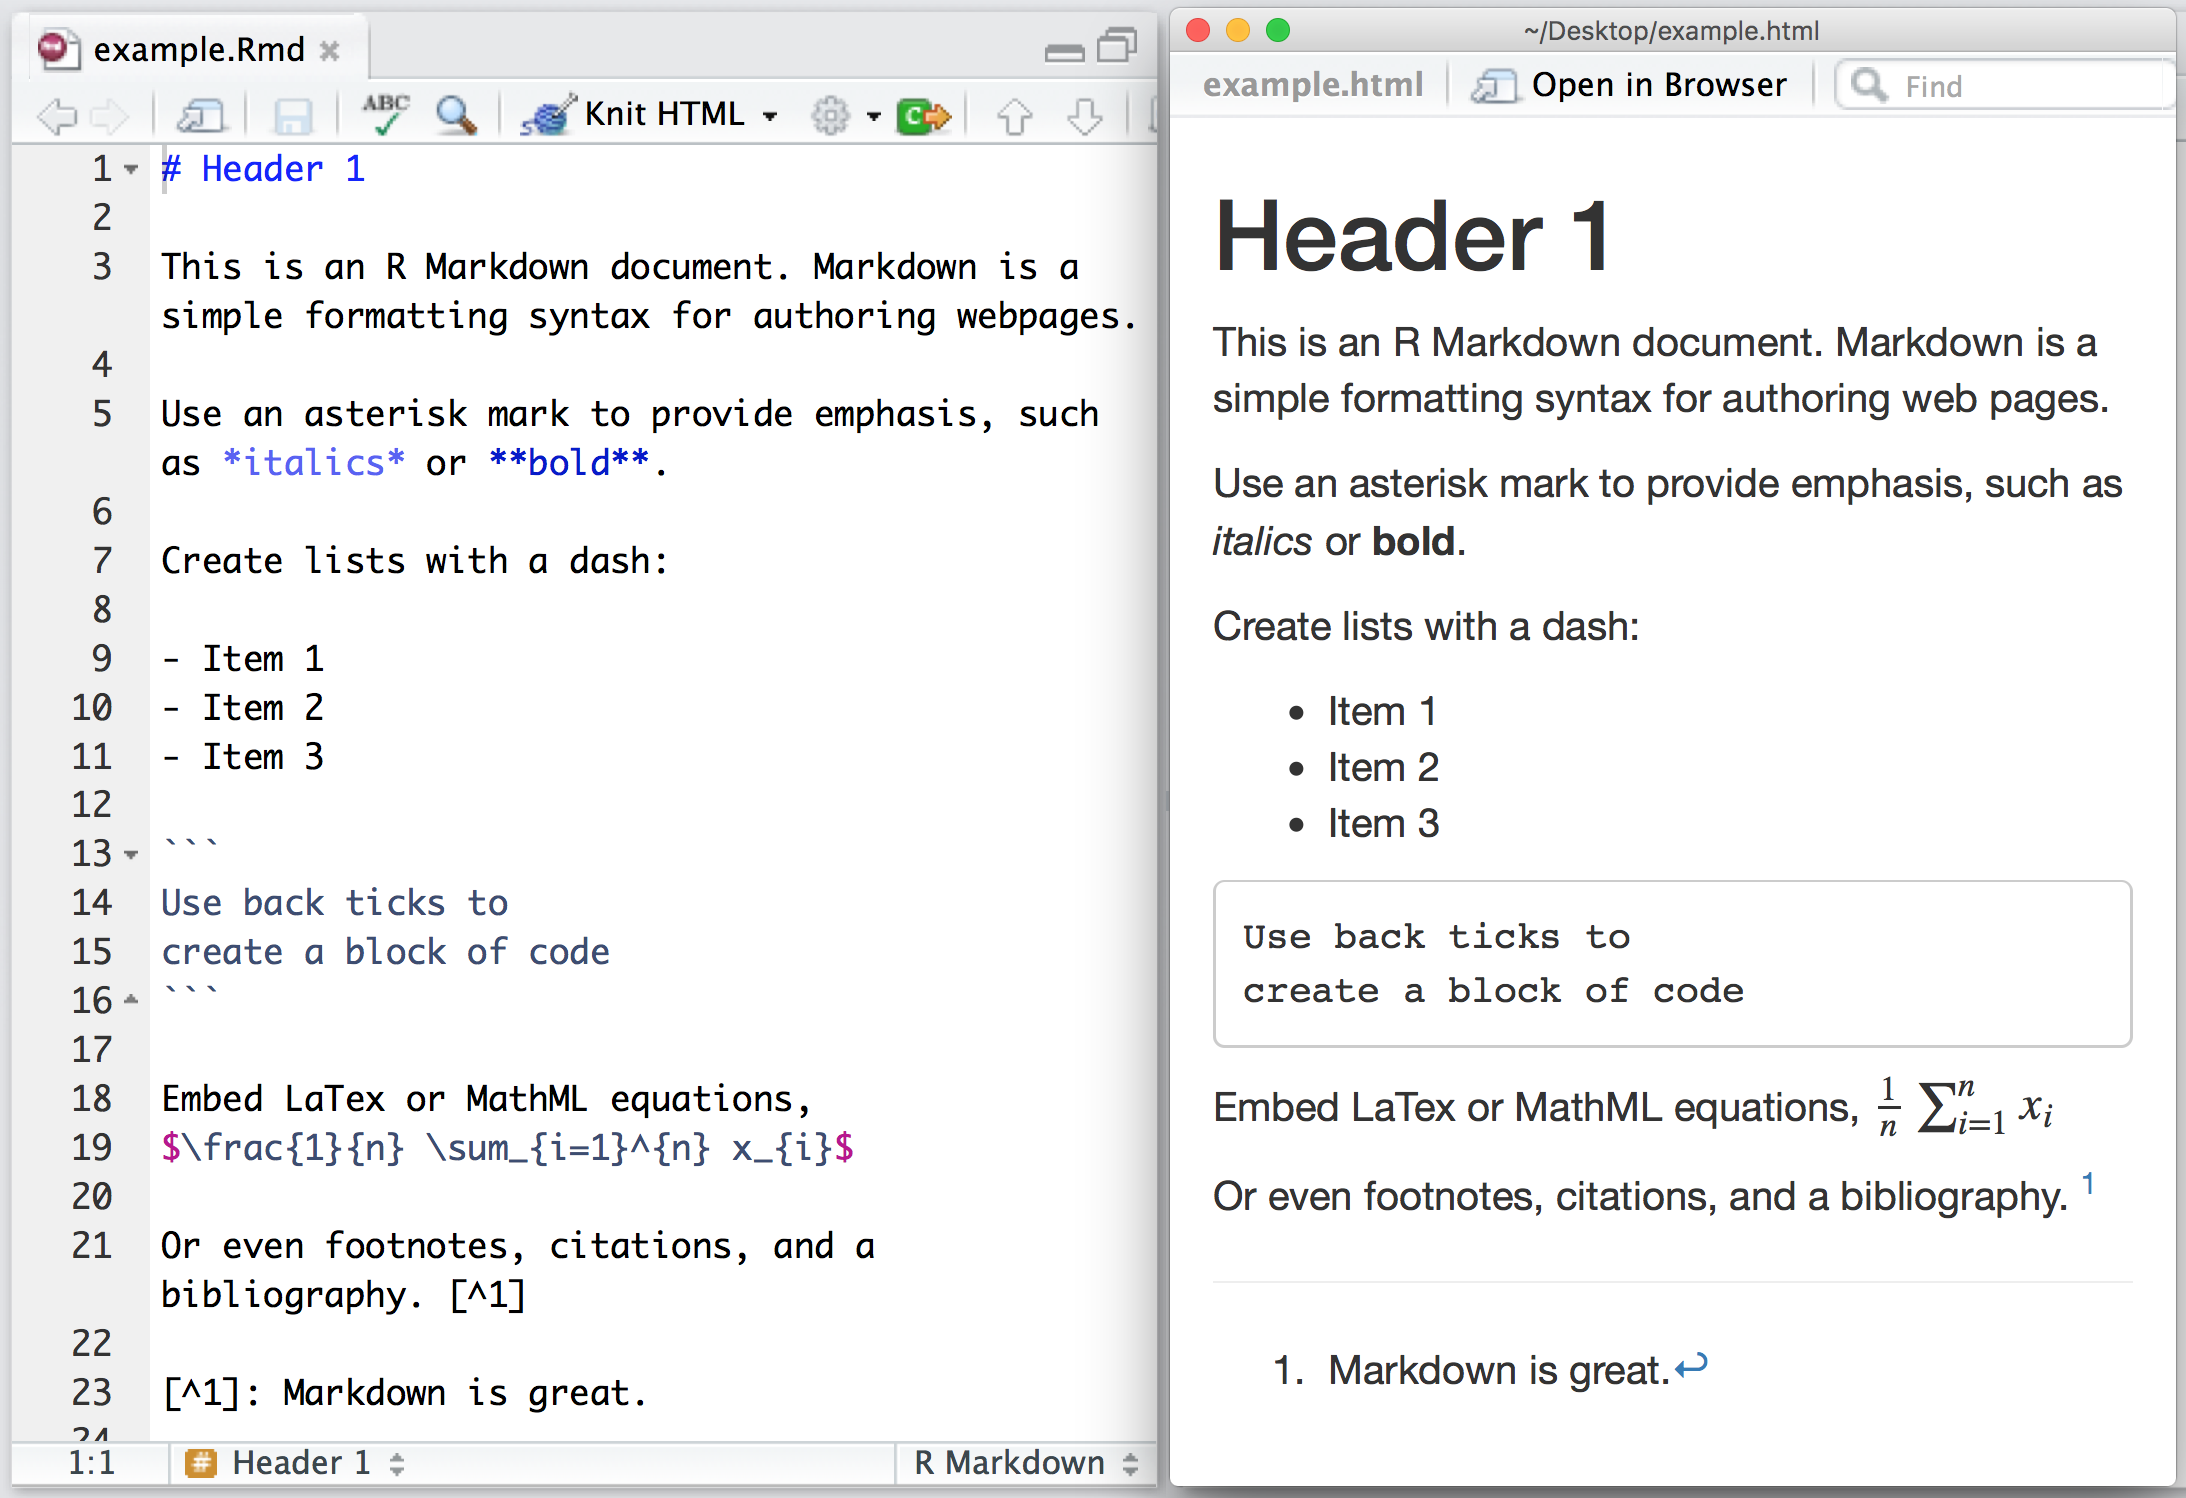
\includegraphics{markdown.png}
\caption{Markdown overview}
\end{figure}
\end{frame}

\begin{frame}{R Code Chunks}
\protect\hypertarget{r-code-chunks}{}
Within an R Markdown file, R Code Chunks can be embedded using the
native Markdown syntax for fenced code regions.

\begin{figure}
\centering
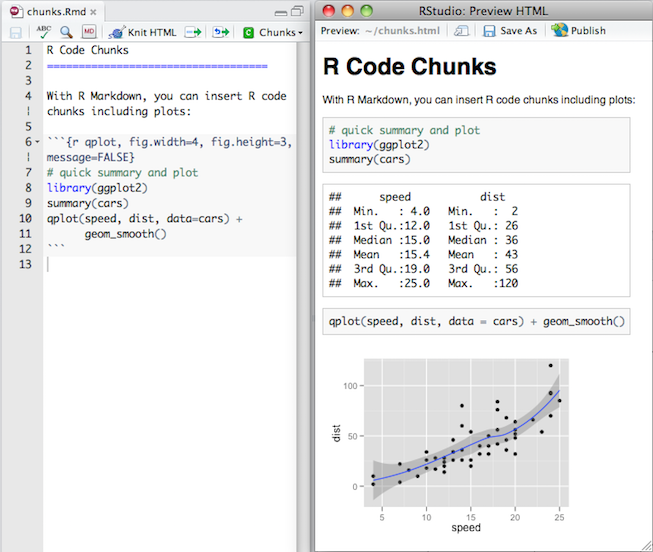
\includegraphics{codechunk.png}
\caption{Code chunks}
\end{figure}
\end{frame}

\begin{frame}{Your turn!}
\protect\hypertarget{your-turn-1}{}
How many code chunks are in your R Markdown document?

What does each code chunk do? You may not understand the R syntax yet,
but you should be able to compare the source file and the output to
answer this question.
\end{frame}

\begin{frame}[fragile]{Inline R Code}
\protect\hypertarget{inline-r-code}{}
You can also evaluate R expressions inline by enclosing the expression
within a single back-tick qualified with \texttt{r}. For example, the
following code: I counted 2 trucks on highway.

Results in this output: ``I counted 2 red trucks on the highway.''
\end{frame}

\begin{frame}{Your turn!}
\protect\hypertarget{your-turn-2}{}
Suppose Sammy works on average 8.37 hours per day, 5 days per week. How
many hours does Sammy work on average per week?

Add a sentence to your document that includes simple inline R code that
answers this question, along the lines of\ldots{}

``Sammy works 8.37 * 5 hours per week, on average.''
\end{frame}

\begin{frame}{Workspaces}
\protect\hypertarget{workspaces}{}
R Markdown workspace and Console workspace are independent of each other

\begin{itemize}
\item
  If you define a variable in your Console and it shows up in the
  Environment tab, it is not going to be automatically included in your
  R Markdown document
\item
  If you define a variable in your R Markdown document, it won't
  automatically be available in your Console
\end{itemize}

{[} Demo {]}

\textbf{Tip:} Use the \emph{Run all previous chunks} in the source file
and \emph{Run current chunk code} functionality in the buttons in each
code chunk to help manage workspaces.
\end{frame}

\begin{frame}{Workspaces and reproducibilty}
\protect\hypertarget{workspaces-and-reproducibilty}{}
\begin{itemize}
\item
  The fact that the two workspaces do not automatically have access to
  the same variables might / will be frustrating at first.
\item
  But this is not a bug, in fact, it's a functionality that helps
  reproducibility, as it ensures that all variables, functions, etc.
  that are being used in the R Markdown document are explicitly defined
  or loaded.
\end{itemize}
\end{frame}

\begin{frame}[fragile]{Your turn!}
\protect\hypertarget{your-turn-3}{}
\begin{enumerate}
\item
  Define \texttt{x\ =\ 2} in the Console. Then, in your Console run
  \texttt{x\ *\ 3}. Does your code run as expected?
\item
  Now, insert a new code chunk in your R Markdown document and in this
  chunk type \texttt{x\ *\ 3} only. Knit your document. Does the
  document compile, or do you get an error? If you get an error, what
  does the error say, and how can you fix it? Implement the fix and Knit
  your document. Make sure you are able to compile without errors before
  you move on.
\end{enumerate}

\textbf{Tip:} Insert a new code chunk bu clicking Chunks \(\rightarrow\)
Insert Chunk.

\begin{enumerate}
\setcounter{enumi}{2}
\item
  Next insert another code chunk in your R Markdown document and define
  \texttt{y\ =\ 4} and calculate \texttt{y\ +\ 5}. Knit your document.
  Does everything work as expected?
\item
  Now run \texttt{y\ +\ 5} in your Console. Does your code run as
  expected or do you get an error? If you get an error, what does the
  error say, and how can you fix it? Implement the fix.
\end{enumerate}
\end{frame}

\begin{frame}{Code chunk options}
\protect\hypertarget{code-chunk-options}{}
\begin{itemize}
\item
  You can hide the code, hide the result, hide warnings, messages, etc.
\item
  Refer to the handy R Markdown
  \href{https://www.rstudio.com/wp-content/uploads/2015/02/rmarkdown-cheatsheet.pdf}{cheatsheet}
\item
  Another good reference:
  \url{http://rmarkdown.rstudio.com/authoring_rcodechunks.html}
\end{itemize}
\end{frame}

\hypertarget{loading-data}{%
\section{Loading data}\label{loading-data}}

\begin{frame}[fragile]{NC DOT Fatal Crashes in North Carolina}
\protect\hypertarget{nc-dot-fatal-crashes-in-north-carolina}{}
\begin{Shaded}
\begin{Highlighting}[]
\FunctionTok{library}\NormalTok{(readr)}
\end{Highlighting}
\end{Shaded}

\begin{verbatim}
## Warning: package 'readr' was built under R version 4.1.3
\end{verbatim}

\begin{Shaded}
\begin{Highlighting}[]
\CommentTok{\#bike \textless{}{-} read\_csv("https://stat.duke.edu/\textasciitilde{}mc301/data/nc\_bike\_crash.csv",                  sep = ";", stringsAsFactors = FALSE, na.strings = c("NA", "", "."))}
\NormalTok{bike}\OtherTok{\textless{}{-}} \FunctionTok{read\_csv}\NormalTok{(}\StringTok{"D:/RepTemplates/data\_analytics/ncbikecrash.csv"}\NormalTok{)}\SpecialCharTok{\%\textgreater{}\%}
  \FunctionTok{tbl\_df}\NormalTok{()}
\end{Highlighting}
\end{Shaded}

\begin{verbatim}
## Warning: `tbl_df()` was deprecated in dplyr 1.0.0.
## Please use `tibble::as_tibble()` instead.
## This warning is displayed once every 8 hours.
## Call `lifecycle::last_lifecycle_warnings()` to see where this warning was generated.
\end{verbatim}

\begin{verbatim}
## New names:
## * `` -> ...1
\end{verbatim}

\begin{verbatim}
## Rows: 7467 Columns: 65
## -- Column specification --------------------------------------------------------
## Delimiter: ","
## chr (48): city, county, region, development, locality, on_road, rural_urban,...
## dbl (17): ...1, object_id, bike_age, driver_age, crash_hour, crash_time, cra...
## 
## i Use `spec()` to retrieve the full column specification for this data.
## i Specify the column types or set `show_col_types = FALSE` to quiet this message.
\end{verbatim}

View the names of variables via

\begin{Shaded}
\begin{Highlighting}[]
\FunctionTok{names}\NormalTok{(bike)}
\end{Highlighting}
\end{Shaded}

\begin{verbatim}
##  [1] "...1"                 "object_id"            "city"                
##  [4] "county"               "region"               "development"         
##  [7] "locality"             "on_road"              "rural_urban"         
## [10] "speed_limit"          "traffic_control"      "weather"             
## [13] "workzone"             "bike_age"             "bike_age_group"      
## [16] "bike_alcohol"         "bike_alcohol_drugs"   "bike_direction"      
## [19] "bike_injury"          "bike_position"        "bike_race"           
## [22] "bike_sex"             "driver_age"           "driver_age_group"    
## [25] "driver_alcohol"       "driver_alcohol_drugs" "driver_est_speed"    
## [28] "driver_injury"        "driver_race"          "driver_sex"          
## [31] "driver_vehicle_type"  "crash_alcohol"        "crash_date"          
## [34] "crash_day"            "crash_group"          "crash_hour"          
## [37] "crash_location"       "crash_month"          "crash_severity"      
## [40] "crash_time"           "crash_type"           "crash_year"          
## [43] "ambulance_req"        "hit_run"              "light_condition"     
## [46] "road_character"       "road_class"           "road_condition"      
## [49] "road_configuration"   "road_defects"         "road_feature"        
## [52] "road_surface"         "num_bikes_ai"         "num_bikes_bi"        
## [55] "num_bikes_ci"         "num_bikes_ki"         "num_bikes_no"        
## [58] "num_bikes_to"         "num_bikes_ui"         "num_lanes"           
## [61] "num_units"            "distance_mi_from"     "frm_road"            
## [64] "rte_invd_cd"          "towrd_road"
\end{verbatim}

and see detailed descriptions at
\url{https://stat.duke.edu/~mc301/data/nc_bike_crash.html}.
\end{frame}

\begin{frame}[fragile]{Aside: Strings (characters) vs factors}
\protect\hypertarget{aside-strings-characters-vs-factors}{}
\begin{itemize}
\item
  By default R will convert character vectors into factors when they are
  included in a data frame.
\item
  Sometimes this is useful, sometimes it isn't -- either way it is
  important to know what type/class you are working with.
\item
  This behavior can be changed using the
  \texttt{stringsAsFactors\ =\ FALSE} when loading a data drame.
\end{itemize}
\end{frame}

\begin{frame}[fragile]{Viewing your data}
\protect\hypertarget{viewing-your-data}{}
\begin{itemize}
\item
  In the Environment, click on the name of the data frame to view it in
  the data viewer
\item
  Use the \texttt{str()} function to compactly display the internal
  \textbf{str}ucture of an R object
\end{itemize}

\begin{Shaded}
\begin{Highlighting}[]
\FunctionTok{str}\NormalTok{(bike)}
\end{Highlighting}
\end{Shaded}

\begin{verbatim}
## tibble [7,467 x 65] (S3: tbl_df/tbl/data.frame)
##  $ ...1                : num [1:7467] 1 2 3 4 5 6 7 8 9 10 ...
##  $ object_id           : num [1:7467] 1686 1674 1673 1687 1653 ...
##  $ city                : chr [1:7467] "None - Rural Crash" "Henderson" "None - Rural Crash" "Whiteville" ...
##  $ county              : chr [1:7467] "Wayne" "Vance" "Lincoln" "Columbus" ...
##  $ region              : chr [1:7467] "Coastal" "Piedmont" "Piedmont" "Coastal" ...
##  $ development         : chr [1:7467] "Farms, Woods, Pastures" "Residential" "Farms, Woods, Pastures" "Commercial" ...
##  $ locality            : chr [1:7467] "Rural (<30% Developed)" "Mixed (30% To 70% Developed)" "Rural (<30% Developed)" "Urban (>70% Developed)" ...
##  $ on_road             : chr [1:7467] "SR 1915" "NICHOLAS ST" "US 321" "W BURKHEAD ST" ...
##  $ rural_urban         : chr [1:7467] "Rural" "Urban" "Rural" "Urban" ...
##  $ speed_limit         : chr [1:7467] "50 - 55  MPH" "30 - 35  MPH" "50 - 55  MPH" "30 - 35  MPH" ...
##  $ traffic_control     : chr [1:7467] "No Control Present" "Stop Sign" "Double Yellow Line, No Passing Zone" "No Control Present" ...
##  $ weather             : chr [1:7467] "Clear" "Clear" "Clear" "Rain" ...
##  $ workzone            : chr [1:7467] "No" "No" "No" "No" ...
##  $ bike_age            : num [1:7467] 52 66 33 52 22 15 41 14 16 54 ...
##  $ bike_age_group      : chr [1:7467] "50-59" "60-69" "30-39" "50-59" ...
##  $ bike_alcohol        : chr [1:7467] "No" "No" "No" "Yes" ...
##  $ bike_alcohol_drugs  : chr [1:7467] NA NA NA NA ...
##  $ bike_direction      : chr [1:7467] "With Traffic" "With Traffic" "With Traffic" NA ...
##  $ bike_injury         : chr [1:7467] "B: Evident Injury" "C: Possible Injury" "C: Possible Injury" "C: Possible Injury" ...
##  $ bike_position       : chr [1:7467] "Bike Lane / Paved Shoulder" "Travel Lane" "Travel Lane" NA ...
##  $ bike_race           : chr [1:7467] "Black" "Black" "White" "Black" ...
##  $ bike_sex            : chr [1:7467] "Male" "Male" "Male" "Male" ...
##  $ driver_age          : num [1:7467] 34 NA 37 55 25 17 NA 50 32 69 ...
##  $ driver_age_group    : chr [1:7467] "30-39" NA "30-39" "50-59" ...
##  $ driver_alcohol      : chr [1:7467] "No" "Missing" "No" "No" ...
##  $ driver_alcohol_drugs: chr [1:7467] NA NA NA NA ...
##  $ driver_est_speed    : chr [1:7467] "51-55 mph" "6-10 mph" "41-45 mph" "11-15 mph" ...
##  $ driver_injury       : chr [1:7467] "O: No Injury" "Unknown Injury" "O: No Injury" "O: No Injury" ...
##  $ driver_race         : chr [1:7467] "White" "Unknown/Missing" "Hispanic" "Black" ...
##  $ driver_sex          : chr [1:7467] "Male" NA "Female" "Male" ...
##  $ driver_vehicle_type : chr [1:7467] "Single Unit Truck (2-Axle, 6-Tire)" NA "Passenger Car" "Passenger Car" ...
##  $ crash_alcohol       : chr [1:7467] "No" "No" "No" "Yes" ...
##  $ crash_date          : chr [1:7467] "11DEC2013" "20NOV2013" "03NOV2013" "14DEC2013" ...
##  $ crash_day           : chr [1:7467] "Wednesday" "Wednesday" "Sunday" "Saturday" ...
##  $ crash_group         : chr [1:7467] "Motorist Overtaking Bicyclist" "Bicyclist Failed to Yield - Sign-Controlled Intersection" "Motorist Overtaking Bicyclist" "Bicyclist Failed to Yield - Signalized Intersection" ...
##  $ crash_hour          : num [1:7467] 6 20 18 18 13 17 17 7 15 2 ...
##  $ crash_location      : chr [1:7467] "Non-Intersection" "Intersection" "Non-Intersection" "Intersection" ...
##  $ crash_month         : chr [1:7467] "December" "November" "November" "December" ...
##  $ crash_severity      : chr [1:7467] "B: Evident Injury" "C: Possible Injury" "C: Possible Injury" "C: Possible Injury" ...
##  $ crash_time          : num [1:7467] 22200 74460 65100 66840 48420 ...
##  $ crash_type          : chr [1:7467] "Motorist Overtaking - Undetected Bicyclist" "Bicyclist Ride Out - Sign-Controlled Intersection" "Motorist Overtaking - Undetected Bicyclist" "Bicyclist Ride Out - Signalized  Intersection" ...
##  $ crash_year          : num [1:7467] 2013 2013 2013 2013 2013 ...
##  $ ambulance_req       : chr [1:7467] "Yes" "No" "Yes" "Yes" ...
##  $ hit_run             : chr [1:7467] "No" "Yes" "No" "No" ...
##  $ light_condition     : chr [1:7467] "Dark - Roadway Not Lighted" NA "Dark - Roadway Not Lighted" "Dark - Lighted Roadway" ...
##  $ road_character      : chr [1:7467] "Straight - Level" "Straight - Level" "Straight - Grade" "Straight - Level" ...
##  $ road_class          : chr [1:7467] "State Secondary Route" "Local Street" "US Route" "Local Street" ...
##  $ road_condition      : chr [1:7467] "Dry" "Dry" "Dry" "Water (Standing, Moving)" ...
##  $ road_configuration  : chr [1:7467] "Two-Way, Not Divided" "Two-Way, Divided, Unprotected Median" "Two-Way, Not Divided" "Two-Way, Not Divided" ...
##  $ road_defects        : chr [1:7467] "None" NA "None" "None" ...
##  $ road_feature        : chr [1:7467] "No Special Feature" "T-Intersection" "No Special Feature" "No Special Feature" ...
##  $ road_surface        : chr [1:7467] "Coarse Asphalt" "Smooth Asphalt" "Smooth Asphalt" "Coarse Asphalt" ...
##  $ num_bikes_ai        : num [1:7467] 0 0 0 0 0 0 0 0 0 0 ...
##  $ num_bikes_bi        : num [1:7467] 0 0 0 0 0 0 0 0 0 0 ...
##  $ num_bikes_ci        : num [1:7467] 0 0 0 0 0 0 0 0 0 0 ...
##  $ num_bikes_ki        : num [1:7467] 0 0 0 0 0 0 0 0 0 0 ...
##  $ num_bikes_no        : num [1:7467] 0 0 0 0 0 0 0 0 0 0 ...
##  $ num_bikes_to        : num [1:7467] 0 0 0 0 0 0 0 0 0 0 ...
##  $ num_bikes_ui        : num [1:7467] 0 0 0 0 0 0 0 0 0 0 ...
##  $ num_lanes           : chr [1:7467] "2 lanes" "2 lanes" "2 lanes" "1 lane" ...
##  $ num_units           : num [1:7467] 2 2 2 2 2 2 2 2 2 2 ...
##  $ distance_mi_from    : num [1:7467] 0 0 0 0 0 0 0 0 0 0 ...
##  $ frm_road            : chr [1:7467] NA NA NA NA ...
##  $ rte_invd_cd         : num [1:7467] 0 0 0 0 0 0 0 0 0 0 ...
##  $ towrd_road          : chr [1:7467] NA NA NA NA ...
\end{verbatim}
\end{frame}

\hypertarget{data-visualization}{%
\section{Data visualization}\label{data-visualization}}

\begin{frame}[fragile]{Data visualization in R}
\protect\hypertarget{data-visualization-in-r}{}
\begin{itemize}
\item
  Using base R functions
\item
  Using the \texttt{ggplot2} package \(\leftarrow\) our focus today
\item
  Using a variety of other packages like \texttt{lattice},
  \texttt{ggvis}, etc.
\end{itemize}
\end{frame}

\begin{frame}[fragile]{The Grammar of Graphics}
\protect\hypertarget{the-grammar-of-graphics}{}
\begin{itemize}
\tightlist
\item
  Visualisation concept created by Wilkinson (1999)

  \begin{itemize}
  \tightlist
  \item
    to define the basic elements of a statistical graphic
  \end{itemize}
\item
  Adapted for R by Wickham (2009) who created the \texttt{ggplot2}
  package

  \begin{itemize}
  \tightlist
  \item
    consistent and compact syntax to describe statistical graphics
  \item
    highly modular as it breaks up graphs into semantic components
  \end{itemize}
\item
  Is not a guide which graph to choose and how to convey information
  best!
\end{itemize}

Source: \url{https://rpubs.com/timwinke/ggplot2workshop}
\end{frame}

\begin{frame}{The Grammar of Graphics - Terminology}
\protect\hypertarget{the-grammar-of-graphics---terminology}{}
A statistical graphic is a\ldots{}

\begin{itemize}
\tightlist
\item
  mapping of \textbf{data}
\item
  to \textbf{aesthetic attributes} (color, size, xy-position)
\item
  using \textbf{geometric objects} (points, lines, bars)
\item
  with data being \textbf{statistically transformed} (summarised,
  log-transformed)
\item
  and mapped onto a specific \textbf{facet} and \textbf{coordinate
  system}
\end{itemize}
\end{frame}

\begin{frame}{Biker age vs.~crash hour}
\protect\hypertarget{biker-age-vs.-crash-hour}{}
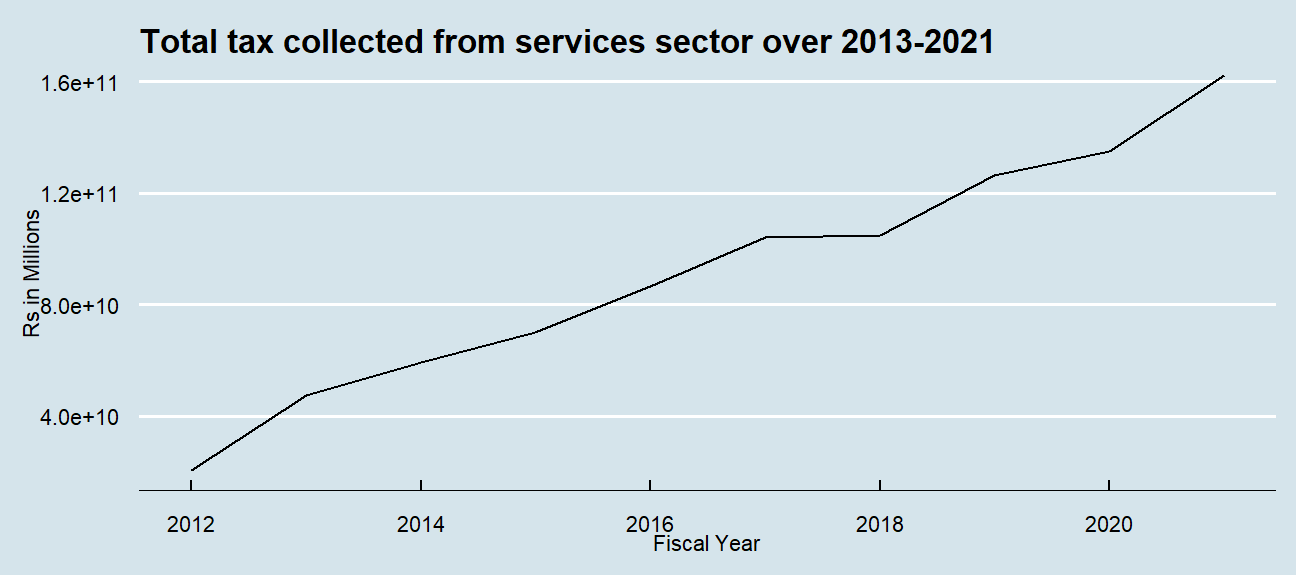
\includegraphics{Learn-R-basics_files/figure-beamer/unnamed-chunk-3-1.pdf}

\begin{itemize}
\tightlist
\item
  Which data is used as an input?
\item
  What geometric objects are chosen for visualization?
\item
  What variables are mapped onto which attributes?
\item
  What type of scales are used to map data to aesthetics?
\item
  Are the variables statistically transformed before plotting?
\end{itemize}
\end{frame}

\begin{frame}[fragile]{Biker age vs.~crash hour - code}
\protect\hypertarget{biker-age-vs.-crash-hour---code}{}
\begin{Shaded}
\begin{Highlighting}[]
\FunctionTok{ggplot}\NormalTok{(}\AttributeTok{data =}\NormalTok{ bike, }\FunctionTok{aes}\NormalTok{(}\AttributeTok{x =}\NormalTok{ crash\_hour, }\AttributeTok{y =}\NormalTok{ bike\_age)) }\SpecialCharTok{+}
  \FunctionTok{geom\_point}\NormalTok{()}
\end{Highlighting}
\end{Shaded}

\begin{verbatim}
## Warning: Removed 209 rows containing missing values (geom_point).
\end{verbatim}

\includegraphics{Learn-R-basics_files/figure-beamer/unnamed-chunk-4-1.pdf}
\end{frame}

\begin{frame}{Altering features}
\protect\hypertarget{altering-features}{}
\includegraphics{Learn-R-basics_files/figure-beamer/unnamed-chunk-5-1.pdf}

\begin{itemize}
\tightlist
\item
  How did the plot change?
\item
  Are these changes based on data (i.e.~can be mapped to variables in
  the dataset) or changes in preferences for geometric objects?
\end{itemize}
\end{frame}

\begin{frame}[fragile]{Altering features - code}
\protect\hypertarget{altering-features---code}{}
\begin{Shaded}
\begin{Highlighting}[]
\FunctionTok{ggplot}\NormalTok{(}\AttributeTok{data =}\NormalTok{ bike, }\FunctionTok{aes}\NormalTok{(}\AttributeTok{x =}\NormalTok{ crash\_hour, }\AttributeTok{y =}\NormalTok{ bike\_age)) }\SpecialCharTok{+}
  \FunctionTok{geom\_point}\NormalTok{(}\AttributeTok{alpha =} \FloatTok{0.5}\NormalTok{, }\AttributeTok{color =} \StringTok{"blue"}\NormalTok{)}
\end{Highlighting}
\end{Shaded}

\begin{verbatim}
## Warning: Removed 209 rows containing missing values (geom_point).
\end{verbatim}

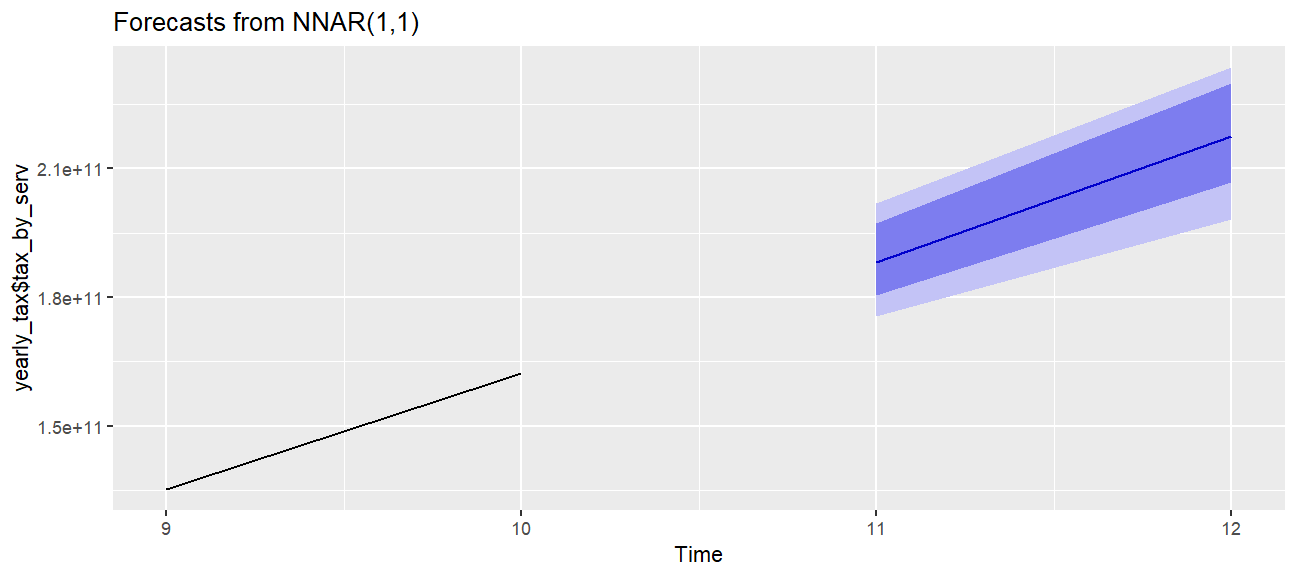
\includegraphics{Learn-R-basics_files/figure-beamer/unnamed-chunk-6-1.pdf}
\end{frame}

\begin{frame}{More alterations}
\protect\hypertarget{more-alterations}{}
\includegraphics{Learn-R-basics_files/figure-beamer/unnamed-chunk-7-1.pdf}

\begin{itemize}
\tightlist
\item
  How did the plot change?
\item
  Are these changes based on data (i.e.~can be mapped to variables in
  the dataset) or changes in preferences for geometric objects?
\end{itemize}
\end{frame}

\begin{frame}[fragile]{More alterations - code}
\protect\hypertarget{more-alterations---code}{}
\begin{Shaded}
\begin{Highlighting}[]
\FunctionTok{ggplot}\NormalTok{(}\AttributeTok{data =}\NormalTok{ bike, }\FunctionTok{aes}\NormalTok{(}\AttributeTok{x =}\NormalTok{ crash\_hour, }\AttributeTok{y =}\NormalTok{ bike\_age, }\AttributeTok{color =}\NormalTok{ ambulance\_req)) }\SpecialCharTok{+}
  \FunctionTok{geom\_point}\NormalTok{(}\AttributeTok{alpha =} \FloatTok{0.5}\NormalTok{) }\SpecialCharTok{+}
  \FunctionTok{facet\_grid}\NormalTok{(. }\SpecialCharTok{\textasciitilde{}}\NormalTok{ bike\_sex)}
\end{Highlighting}
\end{Shaded}

\includegraphics{Learn-R-basics_files/figure-beamer/unnamed-chunk-8-1.pdf}
\end{frame}

\begin{frame}[fragile]{Anatomy of ggplots}
\protect\hypertarget{anatomy-of-ggplots}{}
\begin{verbatim}
ggplot(data = [dataframe], aes(x = [var_x], y = [var_y], 
       color = [var_for_color], fill = [var_for_fill], 
       shape = [var_for_shape])) +
    geom_[some_geom] +
    ... # other options
\end{verbatim}
\end{frame}

\begin{frame}[fragile]{Histograms}
\protect\hypertarget{histograms}{}
\begin{Shaded}
\begin{Highlighting}[]
\FunctionTok{ggplot}\NormalTok{(}\AttributeTok{data =}\NormalTok{ bike, }\FunctionTok{aes}\NormalTok{(}\AttributeTok{x =}\NormalTok{ bike\_age)) }\SpecialCharTok{+}
  \FunctionTok{geom\_histogram}\NormalTok{(}\AttributeTok{binwidth =} \DecValTok{5}\NormalTok{)}
\end{Highlighting}
\end{Shaded}

\includegraphics{Learn-R-basics_files/figure-beamer/unnamed-chunk-9-1.pdf}
\end{frame}

\begin{frame}[fragile]{Boxplots}
\protect\hypertarget{boxplots}{}
\begin{Shaded}
\begin{Highlighting}[]
\FunctionTok{ggplot}\NormalTok{(}\AttributeTok{data =}\NormalTok{ bike, }\FunctionTok{aes}\NormalTok{(}\AttributeTok{y =}\NormalTok{ bike\_age, }\AttributeTok{x =}\NormalTok{ bike\_sex)) }\SpecialCharTok{+}
  \FunctionTok{geom\_boxplot}\NormalTok{()}
\end{Highlighting}
\end{Shaded}

\includegraphics{Learn-R-basics_files/figure-beamer/unnamed-chunk-10-1.pdf}
\end{frame}

\begin{frame}[fragile]{Barplots}
\protect\hypertarget{barplots}{}
\begin{Shaded}
\begin{Highlighting}[]
\FunctionTok{ggplot}\NormalTok{(}\AttributeTok{data =}\NormalTok{ bike, }\FunctionTok{aes}\NormalTok{(}\AttributeTok{x =}\NormalTok{ bike\_injury)) }\SpecialCharTok{+}
  \FunctionTok{geom\_bar}\NormalTok{()}
\end{Highlighting}
\end{Shaded}

\includegraphics{Learn-R-basics_files/figure-beamer/unnamed-chunk-11-1.pdf}
\end{frame}

\begin{frame}[fragile]{Segmented barplots}
\protect\hypertarget{segmented-barplots}{}
\begin{Shaded}
\begin{Highlighting}[]
\FunctionTok{ggplot}\NormalTok{(}\AttributeTok{data =}\NormalTok{ bike, }\FunctionTok{aes}\NormalTok{(}\AttributeTok{x =}\NormalTok{ crash\_location, }\AttributeTok{fill =}\NormalTok{ bike\_injury)) }\SpecialCharTok{+}
  \FunctionTok{geom\_bar}\NormalTok{()}
\end{Highlighting}
\end{Shaded}

\includegraphics{Learn-R-basics_files/figure-beamer/unnamed-chunk-12-1.pdf}
\end{frame}

\begin{frame}[fragile]{Segmented barplots - proportions}
\protect\hypertarget{segmented-barplots---proportions}{}
\begin{Shaded}
\begin{Highlighting}[]
\FunctionTok{ggplot}\NormalTok{(}\AttributeTok{data =}\NormalTok{ bike, }\FunctionTok{aes}\NormalTok{(}\AttributeTok{x =}\NormalTok{ crash\_location, }\AttributeTok{fill =}\NormalTok{ bike\_injury)) }\SpecialCharTok{+}
  \FunctionTok{geom\_bar}\NormalTok{(}\AttributeTok{position=}\StringTok{"fill"}\NormalTok{)}
\end{Highlighting}
\end{Shaded}

\includegraphics{Learn-R-basics_files/figure-beamer/unnamed-chunk-13-1.pdf}
\end{frame}

\begin{frame}[fragile]{More \texttt{ggplot2} resources}
\protect\hypertarget{more-ggplot2-resources}{}
\begin{itemize}
\item
  Visit \url{http://docs.ggplot2.org/current/} for documentation on the
  current version of the \texttt{ggplot2} package. It's full of
  examples!
\item
  Refer to the \texttt{ggplot2}
  \href{https://www.rstudio.com/wp-content/uploads/2015/08/ggplot2-cheatsheet.pdf}{cheatsheet}.
\end{itemize}
\end{frame}

\hypertarget{data-wrangling}{%
\section{Data wrangling}\label{data-wrangling}}

\begin{frame}[fragile]{Data wrangling in R}
\protect\hypertarget{data-wrangling-in-r}{}
\begin{itemize}
\item
  Using base R functions
\item
  Using the \texttt{dplyr} package \(\leftarrow\) our focus today
\item
  Using a variety of other packages like \texttt{plyr}, \texttt{tidyr},
  \texttt{lubridate}, etc.
\end{itemize}
\end{frame}

\begin{frame}[fragile]{Data wrangling with \texttt{dplyr}}
\protect\hypertarget{data-wrangling-with-dplyr}{}
The \texttt{dplyr} package is based on the concepts of functions as
verbs that manipulate data frames:

\begin{itemize}
\tightlist
\item
  \texttt{filter()}: pick rows matching criteria
\item
  \texttt{select()}: pick columns by name
\item
  \texttt{rename()}: rename specific columns
\item
  \texttt{arrange()}: reorder rows
\item
  \texttt{mutate()}: add new variables
\item
  \texttt{transmute()}: create new data frame with variables
\item
  \texttt{sample\_n()} / \texttt{sample\_frac()}: randomly sample rows
\item
  \texttt{summarise()}: reduce variables to values
\end{itemize}
\end{frame}

\begin{frame}{\texttt{dplyr} rules}
\protect\hypertarget{dplyr-rules}{}
\begin{itemize}
\tightlist
\item
  First argument is a data frame
\item
  Subsequent arguments say what to do with data frame
\item
  Always return a data frame
\item
  Avoid modify in place
\end{itemize}
\end{frame}

\begin{frame}{Filter rows with \texttt{filter()}}
\protect\hypertarget{filter-rows-with-filter}{}
\begin{itemize}
\tightlist
\item
  Select a subset of rows in a data frame.
\item
  Easily filter for many conditions at once.
\end{itemize}
\end{frame}

\begin{frame}[fragile]{\texttt{filter()}}
\protect\hypertarget{filter}{}
for crashes in Durham County

\begin{Shaded}
\begin{Highlighting}[]
\NormalTok{bike }\SpecialCharTok{\%\textgreater{}\%}
  \FunctionTok{filter}\NormalTok{(county }\SpecialCharTok{==} \StringTok{"Durham"}\NormalTok{)}
\end{Highlighting}
\end{Shaded}

\begin{verbatim}
## # A tibble: 340 x 65
##     ...1 object_id city   county region development locality on_road rural_urban
##    <dbl>     <dbl> <chr>  <chr>  <chr>  <chr>       <chr>    <chr>   <chr>      
##  1    24      2452 Durham Durham Piedm~ Residential Urban (~ <NA>    Urban      
##  2    28      2441 Durham Durham Piedm~ Commercial  Urban (~ <NA>    Urban      
##  3    37      2466 Durham Durham Piedm~ Commercial  Urban (~ <NA>    Urban      
##  4    63       549 Durham Durham Piedm~ Residential Urban (~ PARK A~ Urban      
##  5    87       598 Durham Durham Piedm~ Residential Urban (~ BELT S~ Urban      
##  6    90       603 Durham Durham Piedm~ Residential Urban (~ HINSON~ Urban      
##  7   144      3974 Durham Durham Piedm~ Commercial  Urban (~ <NA>    Urban      
##  8   231      7134 Durham Durham Piedm~ Commercial  Urban (~ <NA>    Urban      
##  9   336      1670 Durham Durham Piedm~ Commercial  Urban (~ INFINI~ Urban      
## 10   351      1773 Durham Durham Piedm~ Residential Urban (~ <NA>    Urban      
## # ... with 330 more rows, and 56 more variables: speed_limit <chr>,
## #   traffic_control <chr>, weather <chr>, workzone <chr>, bike_age <dbl>,
## #   bike_age_group <chr>, bike_alcohol <chr>, bike_alcohol_drugs <chr>,
## #   bike_direction <chr>, bike_injury <chr>, bike_position <chr>,
## #   bike_race <chr>, bike_sex <chr>, driver_age <dbl>, driver_age_group <chr>,
## #   driver_alcohol <chr>, driver_alcohol_drugs <chr>, driver_est_speed <chr>,
## #   driver_injury <chr>, driver_race <chr>, driver_sex <chr>, ...
\end{verbatim}
\end{frame}

\begin{frame}[fragile]{\texttt{filter()}}
\protect\hypertarget{filter-1}{}
for crashes in Durham County where biker was \textless{} 10 yrs old

\begin{Shaded}
\begin{Highlighting}[]
\NormalTok{bike }\SpecialCharTok{\%\textgreater{}\%}
  \FunctionTok{filter}\NormalTok{(county }\SpecialCharTok{==} \StringTok{"Durham"}\NormalTok{, bike\_age }\SpecialCharTok{\textless{}} \DecValTok{10}\NormalTok{)}
\end{Highlighting}
\end{Shaded}

\begin{verbatim}
## # A tibble: 27 x 65
##     ...1 object_id city   county region development locality on_road rural_urban
##    <dbl>     <dbl> <chr>  <chr>  <chr>  <chr>       <chr>    <chr>   <chr>      
##  1    24      2452 Durham Durham Piedm~ Residential Urban (~ <NA>    Urban      
##  2    63       549 Durham Durham Piedm~ Residential Urban (~ PARK A~ Urban      
##  3   519      2279 Durham Durham Piedm~ Residential Urban (~ <NA>    Urban      
##  4   827      2431 Durham Durham Piedm~ Residential Urban (~ <NA>    Urban      
##  5  1072      4611 Durham Durham Piedm~ Residential Urban (~ <NA>    Urban      
##  6  1147       950 Durham Durham Piedm~ Residential Urban (~ BERWYN~ Urban      
##  7  1767      6773 Durham Durham Piedm~ Residential Urban (~ <NA>    Urban      
##  8  2429      4106 Durham Durham Piedm~ Residential Urban (~ <NA>    Urban      
##  9  3337      6485 Durham Durham Piedm~ Residential Mixed (~ <NA>    Urban      
## 10  3349      6591 Durham Durham Piedm~ Residential Urban (~ <NA>    Urban      
## # ... with 17 more rows, and 56 more variables: speed_limit <chr>,
## #   traffic_control <chr>, weather <chr>, workzone <chr>, bike_age <dbl>,
## #   bike_age_group <chr>, bike_alcohol <chr>, bike_alcohol_drugs <chr>,
## #   bike_direction <chr>, bike_injury <chr>, bike_position <chr>,
## #   bike_race <chr>, bike_sex <chr>, driver_age <dbl>, driver_age_group <chr>,
## #   driver_alcohol <chr>, driver_alcohol_drugs <chr>, driver_est_speed <chr>,
## #   driver_injury <chr>, driver_race <chr>, driver_sex <chr>, ...
\end{verbatim}
\end{frame}

\begin{frame}[fragile]{Commonly used logical operators in R}
\protect\hypertarget{commonly-used-logical-operators-in-r}{}
\begin{longtable}[]{@{}ll@{}}
\toprule
operator & definition \\
\midrule
\endhead
\texttt{\textless{}} & less than \\
\texttt{\textless{}=} & less than or equal to \\
\texttt{\textgreater{}} & greater than \\
\texttt{\textgreater{}=} & greater than or equal to \\
\texttt{==} & exactly equal to \\
\texttt{!=} & not equal to \\
\texttt{x\ \textbar{}\ y} & \texttt{x} OR \texttt{y} \\
\texttt{x\ \&\ y} & \texttt{x} AND \texttt{y} \\
\bottomrule
\end{longtable}
\end{frame}

\begin{frame}[fragile]{Commonly used logical operators in R}
\protect\hypertarget{commonly-used-logical-operators-in-r-1}{}
\begin{longtable}[]{@{}ll@{}}
\toprule
operator & definition \\
\midrule
\endhead
\texttt{is.na(x)} & test if \texttt{x} is \texttt{NA} \\
\texttt{!is.na(x)} & test if \texttt{x} is not \texttt{NA} \\
\texttt{x\ \%in\%\ y} & test if \texttt{x} is in \texttt{y} \\
\texttt{!(x\ \%in\%\ y)} & test if \texttt{x} is not in \texttt{y} \\
\texttt{!x} & not \texttt{x} \\
\bottomrule
\end{longtable}
\end{frame}

\begin{frame}[fragile]{Aside: real data is messy!}
\protect\hypertarget{aside-real-data-is-messy}{}
What in the world does a \texttt{bike\_age\_group} of \texttt{10-Jun} or
\texttt{15-Nov} mean?

\begin{Shaded}
\begin{Highlighting}[]
\NormalTok{bike }\SpecialCharTok{\%\textgreater{}\%}
  \FunctionTok{group\_by}\NormalTok{(bike\_age\_group) }\SpecialCharTok{\%\textgreater{}\%}
  \FunctionTok{summarise}\NormalTok{(}\AttributeTok{crash\_count =} \FunctionTok{n}\NormalTok{())}
\end{Highlighting}
\end{Shaded}

\begin{verbatim}
## # A tibble: 12 x 2
##    bike_age_group crash_count
##    <chr>                <int>
##  1 0-5                     86
##  2 11-15                  933
##  3 16-19                  794
##  4 20-24                  910
##  5 25-29                  578
##  6 30-39                  881
##  7 40-49                 1144
##  8 50-59                 1013
##  9 6-10                   537
## 10 60-69                  382
## 11 70+                     96
## 12 <NA>                   113
\end{verbatim}
\end{frame}

\begin{frame}[fragile]{Careful data scientists clean up their data
first!}
\protect\hypertarget{careful-data-scientists-clean-up-their-data-first}{}
\begin{itemize}
\tightlist
\item
  We're going to need to do some text parsing to clean up these data

  \begin{itemize}
  \tightlist
  \item
    \texttt{10-Jun} should be \texttt{6-10}
  \item
    \texttt{15-Nov} should be \texttt{11-15}
  \end{itemize}
\item
  New R package: \texttt{stringr}
\end{itemize}
\end{frame}

\begin{frame}[fragile]{Install and load: \texttt{stringr}}
\protect\hypertarget{install-and-load-stringr}{}
\begin{itemize}
\tightlist
\item
  Install:
\end{itemize}

\begin{Shaded}
\begin{Highlighting}[]
\CommentTok{\#install.packages("stringr")}
\end{Highlighting}
\end{Shaded}

\begin{itemize}
\tightlist
\item
  Load:
\end{itemize}

\begin{Shaded}
\begin{Highlighting}[]
\FunctionTok{library}\NormalTok{(stringr)}
\end{Highlighting}
\end{Shaded}

\begin{itemize}
\tightlist
\item
  Package reference: Most R packages come with a vignette that describe
  in detail what each function does and how to use them, they're
  incredibly useful resources (in addition to other worked out examples
  on the web)
  \url{https://cran.r-project.org/web/packages/stringr/vignettes/stringr.html}
\end{itemize}
\end{frame}

\begin{frame}[fragile]{Replace with \texttt{str\_replace()} and add new
variables with \texttt{mutate()}}
\protect\hypertarget{replace-with-str_replace-and-add-new-variables-with-mutate}{}
\begin{itemize}
\tightlist
\item
  Remember we want to do the following in the \texttt{bike\_age\_group}
  variable: \texttt{10-Jun} should be \texttt{6-10} and \texttt{15-Nov}
  should be \texttt{11-15}
\end{itemize}

\begin{Shaded}
\begin{Highlighting}[]
\NormalTok{bike }\OtherTok{\textless{}{-}}\NormalTok{ bike }\SpecialCharTok{\%\textgreater{}\%}
  \FunctionTok{mutate}\NormalTok{(}\AttributeTok{bike\_age\_group =} \FunctionTok{str\_replace}\NormalTok{(bike\_age\_group, }\StringTok{"10{-}Jun"}\NormalTok{, }\StringTok{"6{-}10"}\NormalTok{)) }\SpecialCharTok{\%\textgreater{}\%}
  \FunctionTok{mutate}\NormalTok{(}\AttributeTok{bike\_age\_group =} \FunctionTok{str\_replace}\NormalTok{(bike\_age\_group, }\StringTok{"15{-}Nov"}\NormalTok{, }\StringTok{"11{-}15"}\NormalTok{))}
\end{Highlighting}
\end{Shaded}

\begin{itemize}
\tightlist
\item
  Note that we're overwriting existing data and columns, so be careful!

  \begin{itemize}
  \tightlist
  \item
    But remember, it's easy to revert if you make a mistake since we
    didn't touch the raw data, we can always reload it and start over
  \end{itemize}
\end{itemize}
\end{frame}

\begin{frame}[fragile]{Check before you move on}
\protect\hypertarget{check-before-you-move-on}{}
Always check your changes and confirm code did what you wanted it to do

\begin{Shaded}
\begin{Highlighting}[]
\NormalTok{bike }\SpecialCharTok{\%\textgreater{}\%}
  \FunctionTok{group\_by}\NormalTok{(bike\_age\_group) }\SpecialCharTok{\%\textgreater{}\%}
  \FunctionTok{summarise}\NormalTok{(}\AttributeTok{count =} \FunctionTok{n}\NormalTok{())}
\end{Highlighting}
\end{Shaded}

\begin{verbatim}
## # A tibble: 12 x 2
##    bike_age_group count
##    <chr>          <int>
##  1 0-5               86
##  2 11-15            933
##  3 16-19            794
##  4 20-24            910
##  5 25-29            578
##  6 30-39            881
##  7 40-49           1144
##  8 50-59           1013
##  9 6-10             537
## 10 60-69            382
## 11 70+               96
## 12 <NA>             113
\end{verbatim}
\end{frame}

\begin{frame}[fragile]{\texttt{slice()} for certain row numbers}
\protect\hypertarget{slice-for-certain-row-numbers}{}
First five

\begin{Shaded}
\begin{Highlighting}[]
\NormalTok{bike }\SpecialCharTok{\%\textgreater{}\%}
  \FunctionTok{slice}\NormalTok{(}\DecValTok{1}\SpecialCharTok{:}\DecValTok{5}\NormalTok{)}
\end{Highlighting}
\end{Shaded}

\begin{verbatim}
## # A tibble: 5 x 65
##    ...1 object_id city    county region development locality on_road rural_urban
##   <dbl>     <dbl> <chr>   <chr>  <chr>  <chr>       <chr>    <chr>   <chr>      
## 1     1      1686 None -~ Wayne  Coast~ Farms, Woo~ Rural (~ SR 1915 Rural      
## 2     2      1674 Hender~ Vance  Piedm~ Residential Mixed (~ NICHOL~ Urban      
## 3     3      1673 None -~ Linco~ Piedm~ Farms, Woo~ Rural (~ US 321  Rural      
## 4     4      1687 Whitev~ Colum~ Coast~ Commercial  Urban (~ W BURK~ Urban      
## 5     5      1653 Wilmin~ New H~ Coast~ Residential Urban (~ RACINE~ Urban      
## # ... with 56 more variables: speed_limit <chr>, traffic_control <chr>,
## #   weather <chr>, workzone <chr>, bike_age <dbl>, bike_age_group <chr>,
## #   bike_alcohol <chr>, bike_alcohol_drugs <chr>, bike_direction <chr>,
## #   bike_injury <chr>, bike_position <chr>, bike_race <chr>, bike_sex <chr>,
## #   driver_age <dbl>, driver_age_group <chr>, driver_alcohol <chr>,
## #   driver_alcohol_drugs <chr>, driver_est_speed <chr>, driver_injury <chr>,
## #   driver_race <chr>, driver_sex <chr>, driver_vehicle_type <chr>, ...
\end{verbatim}
\end{frame}

\begin{frame}[fragile]{\texttt{slice()} for certain row numbers}
\protect\hypertarget{slice-for-certain-row-numbers-1}{}
Last five

\begin{Shaded}
\begin{Highlighting}[]
\NormalTok{last\_row }\OtherTok{\textless{}{-}} \FunctionTok{nrow}\NormalTok{(bike)}
\NormalTok{bike }\SpecialCharTok{\%\textgreater{}\%}
  \FunctionTok{slice}\NormalTok{((last\_row}\DecValTok{{-}4}\NormalTok{)}\SpecialCharTok{:}\NormalTok{last\_row)}
\end{Highlighting}
\end{Shaded}

\begin{verbatim}
## # A tibble: 5 x 65
##    ...1 object_id city    county region development locality on_road rural_urban
##   <dbl>     <dbl> <chr>   <chr>  <chr>  <chr>       <chr>    <chr>   <chr>      
## 1  7463      6989 High P~ Guilf~ Piedm~ Residential Urban (~ <NA>    Urban      
## 2  7464      6991 Wilmin~ New H~ Coast~ Residential Urban (~ <NA>    Urban      
## 3  7465      6995 Kinston Lenoir Coast~ Commercial  Urban (~ <NA>    Urban      
## 4  7466      6998 Fayett~ Cumbe~ Coast~ Residential Urban (~ <NA>    Urban      
## 5  7467      7000 None -~ Onslow Coast~ Farms, Woo~ Rural (~ <NA>    Rural      
## # ... with 56 more variables: speed_limit <chr>, traffic_control <chr>,
## #   weather <chr>, workzone <chr>, bike_age <dbl>, bike_age_group <chr>,
## #   bike_alcohol <chr>, bike_alcohol_drugs <chr>, bike_direction <chr>,
## #   bike_injury <chr>, bike_position <chr>, bike_race <chr>, bike_sex <chr>,
## #   driver_age <dbl>, driver_age_group <chr>, driver_alcohol <chr>,
## #   driver_alcohol_drugs <chr>, driver_est_speed <chr>, driver_injury <chr>,
## #   driver_race <chr>, driver_sex <chr>, driver_vehicle_type <chr>, ...
\end{verbatim}
\end{frame}

\begin{frame}[fragile]{\texttt{select()} to keep only the variables you
mention}
\protect\hypertarget{select-to-keep-only-the-variables-you-mention}{}
\begin{Shaded}
\begin{Highlighting}[]
\NormalTok{bike }\SpecialCharTok{\%\textgreater{}\%}
  \FunctionTok{select}\NormalTok{(crash\_location, hit\_run) }\SpecialCharTok{\%\textgreater{}\%}
  \FunctionTok{table}\NormalTok{()}
\end{Highlighting}
\end{Shaded}

\begin{verbatim}
##                       hit_run
## crash_location           No  Yes
##   Intersection         2878  352
##   Intersection-Related  369   72
##   Non-Intersection     2876  587
##   Non-Roadway           281   38
##   Unknown Location        3    7
\end{verbatim}
\end{frame}

\begin{frame}[fragile]{or \texttt{select()}to exclude variables}
\protect\hypertarget{or-selectto-exclude-variables}{}
\begin{Shaded}
\begin{Highlighting}[]
\NormalTok{bike }\SpecialCharTok{\%\textgreater{}\%}
  \FunctionTok{select}\NormalTok{(}\SpecialCharTok{{-}}\NormalTok{object\_id)}
\end{Highlighting}
\end{Shaded}

\begin{verbatim}
## # A tibble: 7,467 x 64
##     ...1 city             county region development locality on_road rural_urban
##    <dbl> <chr>            <chr>  <chr>  <chr>       <chr>    <chr>   <chr>      
##  1     1 None - Rural Cr~ Wayne  Coast~ Farms, Woo~ Rural (~ SR 1915 Rural      
##  2     2 Henderson        Vance  Piedm~ Residential Mixed (~ NICHOL~ Urban      
##  3     3 None - Rural Cr~ Linco~ Piedm~ Farms, Woo~ Rural (~ US 321  Rural      
##  4     4 Whiteville       Colum~ Coast~ Commercial  Urban (~ W BURK~ Urban      
##  5     5 Wilmington       New H~ Coast~ Residential Urban (~ RACINE~ Urban      
##  6     6 None - Rural Cr~ Robes~ Coast~ Farms, Woo~ Rural (~ SR 1513 Rural      
##  7     7 None - Rural Cr~ Richm~ Piedm~ Residential Mixed (~ SR 1903 Rural      
##  8     8 Raleigh          Wake   Piedm~ Commercial  Urban (~ PERSON~ Urban      
##  9     9 Whiteville       Colum~ Coast~ Residential Rural (~ FLOWER~ Urban      
## 10    10 New Bern         Craven Coast~ Residential Urban (~ SUTTON~ Urban      
## # ... with 7,457 more rows, and 56 more variables: speed_limit <chr>,
## #   traffic_control <chr>, weather <chr>, workzone <chr>, bike_age <dbl>,
## #   bike_age_group <chr>, bike_alcohol <chr>, bike_alcohol_drugs <chr>,
## #   bike_direction <chr>, bike_injury <chr>, bike_position <chr>,
## #   bike_race <chr>, bike_sex <chr>, driver_age <dbl>, driver_age_group <chr>,
## #   driver_alcohol <chr>, driver_alcohol_drugs <chr>, driver_est_speed <chr>,
## #   driver_injury <chr>, driver_race <chr>, driver_sex <chr>, ...
\end{verbatim}
\end{frame}

\begin{frame}[fragile]{\texttt{rename()} specific columns}
\protect\hypertarget{rename-specific-columns}{}
Correct typos and rename to make variable names shorter and/or more
informative

\begin{itemize}
\tightlist
\item
  Original names:
\end{itemize}

\begin{Shaded}
\begin{Highlighting}[]
\FunctionTok{names}\NormalTok{(bike)}
\end{Highlighting}
\end{Shaded}

\begin{verbatim}
##  [1] "...1"                 "object_id"            "city"                
##  [4] "county"               "region"               "development"         
##  [7] "locality"             "on_road"              "rural_urban"         
## [10] "speed_limit"          "traffic_control"      "weather"             
## [13] "workzone"             "bike_age"             "bike_age_group"      
## [16] "bike_alcohol"         "bike_alcohol_drugs"   "bike_direction"      
## [19] "bike_injury"          "bike_position"        "bike_race"           
## [22] "bike_sex"             "driver_age"           "driver_age_group"    
## [25] "driver_alcohol"       "driver_alcohol_drugs" "driver_est_speed"    
## [28] "driver_injury"        "driver_race"          "driver_sex"          
## [31] "driver_vehicle_type"  "crash_alcohol"        "crash_date"          
## [34] "crash_day"            "crash_group"          "crash_hour"          
## [37] "crash_location"       "crash_month"          "crash_severity"      
## [40] "crash_time"           "crash_type"           "crash_year"          
## [43] "ambulance_req"        "hit_run"              "light_condition"     
## [46] "road_character"       "road_class"           "road_condition"      
## [49] "road_configuration"   "road_defects"         "road_feature"        
## [52] "road_surface"         "num_bikes_ai"         "num_bikes_bi"        
## [55] "num_bikes_ci"         "num_bikes_ki"         "num_bikes_no"        
## [58] "num_bikes_to"         "num_bikes_ui"         "num_lanes"           
## [61] "num_units"            "distance_mi_from"     "frm_road"            
## [64] "rte_invd_cd"          "towrd_road"
\end{verbatim}

\begin{itemize}
\tightlist
\item
  Rename \texttt{Speed\_Limi} to \texttt{Speed\_Limit}:
\end{itemize}

\begin{Shaded}
\begin{Highlighting}[]
\CommentTok{\#bike \textless{}{-} bike \%\textgreater{}\%}
\CommentTok{\#  rename(speed\_limit = Speed\_Limi)\#\# Its already in speed\_limit}
\end{Highlighting}
\end{Shaded}
\end{frame}

\begin{frame}[fragile]{Check before you move on}
\protect\hypertarget{check-before-you-move-on-1}{}
Always check your changes and confirm code did what you wanted it to do

\begin{Shaded}
\begin{Highlighting}[]
\FunctionTok{names}\NormalTok{(bike)}
\end{Highlighting}
\end{Shaded}

\begin{verbatim}
##  [1] "...1"                 "object_id"            "city"                
##  [4] "county"               "region"               "development"         
##  [7] "locality"             "on_road"              "rural_urban"         
## [10] "speed_limit"          "traffic_control"      "weather"             
## [13] "workzone"             "bike_age"             "bike_age_group"      
## [16] "bike_alcohol"         "bike_alcohol_drugs"   "bike_direction"      
## [19] "bike_injury"          "bike_position"        "bike_race"           
## [22] "bike_sex"             "driver_age"           "driver_age_group"    
## [25] "driver_alcohol"       "driver_alcohol_drugs" "driver_est_speed"    
## [28] "driver_injury"        "driver_race"          "driver_sex"          
## [31] "driver_vehicle_type"  "crash_alcohol"        "crash_date"          
## [34] "crash_day"            "crash_group"          "crash_hour"          
## [37] "crash_location"       "crash_month"          "crash_severity"      
## [40] "crash_time"           "crash_type"           "crash_year"          
## [43] "ambulance_req"        "hit_run"              "light_condition"     
## [46] "road_character"       "road_class"           "road_condition"      
## [49] "road_configuration"   "road_defects"         "road_feature"        
## [52] "road_surface"         "num_bikes_ai"         "num_bikes_bi"        
## [55] "num_bikes_ci"         "num_bikes_ki"         "num_bikes_no"        
## [58] "num_bikes_to"         "num_bikes_ui"         "num_lanes"           
## [61] "num_units"            "distance_mi_from"     "frm_road"            
## [64] "rte_invd_cd"          "towrd_road"
\end{verbatim}
\end{frame}

\begin{frame}[fragile]{\texttt{summarise()} in a new data frame}
\protect\hypertarget{summarise-in-a-new-data-frame}{}
\begin{Shaded}
\begin{Highlighting}[]
\NormalTok{bike }\SpecialCharTok{\%\textgreater{}\%}
  \FunctionTok{group\_by}\NormalTok{(bike\_age\_group) }\SpecialCharTok{\%\textgreater{}\%}
  \FunctionTok{summarise}\NormalTok{(}\AttributeTok{crash\_count =} \FunctionTok{n}\NormalTok{()) }\SpecialCharTok{\%\textgreater{}\%}
  \FunctionTok{arrange}\NormalTok{(crash\_count)}
\end{Highlighting}
\end{Shaded}

\begin{verbatim}
## # A tibble: 12 x 2
##    bike_age_group crash_count
##    <chr>                <int>
##  1 0-5                     86
##  2 70+                     96
##  3 <NA>                   113
##  4 60-69                  382
##  5 6-10                   537
##  6 25-29                  578
##  7 16-19                  794
##  8 30-39                  881
##  9 20-24                  910
## 10 11-15                  933
## 11 50-59                 1013
## 12 40-49                 1144
\end{verbatim}
\end{frame}

\begin{frame}[fragile]{and \texttt{arrange()} to order rows}
\protect\hypertarget{and-arrange-to-order-rows}{}
\begin{Shaded}
\begin{Highlighting}[]
\NormalTok{bike }\SpecialCharTok{\%\textgreater{}\%}
  \FunctionTok{group\_by}\NormalTok{(bike\_age\_group) }\SpecialCharTok{\%\textgreater{}\%}
  \FunctionTok{summarise}\NormalTok{(}\AttributeTok{crash\_count =} \FunctionTok{n}\NormalTok{()) }\SpecialCharTok{\%\textgreater{}\%}
  \FunctionTok{arrange}\NormalTok{(}\FunctionTok{desc}\NormalTok{(crash\_count))}
\end{Highlighting}
\end{Shaded}

\begin{verbatim}
## # A tibble: 12 x 2
##    bike_age_group crash_count
##    <chr>                <int>
##  1 40-49                 1144
##  2 50-59                 1013
##  3 11-15                  933
##  4 20-24                  910
##  5 30-39                  881
##  6 16-19                  794
##  7 25-29                  578
##  8 6-10                   537
##  9 60-69                  382
## 10 <NA>                   113
## 11 70+                     96
## 12 0-5                     86
\end{verbatim}
\end{frame}

\begin{frame}[fragile]{Select rows with \texttt{sample\_n()} or
\texttt{sample\_frac()}}
\protect\hypertarget{select-rows-with-sample_n-or-sample_frac}{}
\begin{itemize}
\tightlist
\item
  \texttt{sample\_n()}: randomly sample 5 observations
\end{itemize}

\begin{Shaded}
\begin{Highlighting}[]
\NormalTok{bike\_n5 }\OtherTok{\textless{}{-}}\NormalTok{ bike }\SpecialCharTok{\%\textgreater{}\%}
  \FunctionTok{sample\_n}\NormalTok{(}\DecValTok{5}\NormalTok{, }\AttributeTok{replace =} \ConstantTok{FALSE}\NormalTok{)}
\FunctionTok{dim}\NormalTok{(bike\_n5)}
\end{Highlighting}
\end{Shaded}

\begin{verbatim}
## [1]  5 65
\end{verbatim}

\begin{itemize}
\tightlist
\item
  \texttt{sample\_frac()}: randomly sample 20\% of observations
\end{itemize}

\begin{Shaded}
\begin{Highlighting}[]
\NormalTok{bike\_perc20 }\OtherTok{\textless{}{-}}\NormalTok{bike }\SpecialCharTok{\%\textgreater{}\%}
  \FunctionTok{sample\_frac}\NormalTok{(}\FloatTok{0.2}\NormalTok{, }\AttributeTok{replace =} \ConstantTok{FALSE}\NormalTok{)}
\FunctionTok{dim}\NormalTok{(bike\_perc20)}
\end{Highlighting}
\end{Shaded}

\begin{verbatim}
## [1] 1493   65
\end{verbatim}
\end{frame}

\begin{frame}[fragile]{More \texttt{dplyr} resources}
\protect\hypertarget{more-dplyr-resources}{}
\begin{itemize}
\item
  Visit
  \url{https://cran.r-project.org/web/packages/dplyr/vignettes/introduction.html}
  for the package vignette.
\item
  Refer to the \texttt{dplyr}
  \href{https://www.rstudio.com/wp-content/uploads/2015/02/data-wrangling-cheatsheet.pdf}{cheatsheet}.
\end{itemize}
\end{frame}

\hypertarget{basic-r-syntax}{%
\section{Basic R syntax}\label{basic-r-syntax}}

\begin{frame}[fragile]{Few important R syntax notes}
\protect\hypertarget{few-important-r-syntax-notes}{}
For when not working with \texttt{dplyr} or \texttt{ggplot2}

\begin{itemize}
\item
  Refer to a variable in a dataset as \texttt{bike\$crash\_location}
\item
  Access any element in a dataframe using square brackets
\end{itemize}

\begin{Shaded}
\begin{Highlighting}[]
\NormalTok{bike[}\DecValTok{1}\NormalTok{,}\DecValTok{5}\NormalTok{] }\CommentTok{\# row 1, column 5}
\end{Highlighting}
\end{Shaded}

\begin{verbatim}
## # A tibble: 1 x 1
##   region 
##   <chr>  
## 1 Coastal
\end{verbatim}

\begin{verbatim}
- For all observations in row 1: `bike[1, ]`
- For all observations in column 5: `bike[, 5]`
\end{verbatim}
\end{frame}

\hypertarget{whats-next}{%
\section{What's next?}\label{whats-next}}

\begin{frame}{Want more R?}
\protect\hypertarget{want-more-r}{}
\begin{itemize}
\tightlist
\item
  Local install

  \begin{itemize}
  \tightlist
  \item
    R: \url{https://cran.r-project.org/}
  \item
    RStudio: \url{https://www.rstudio.com/products/RStudio/\#Desktop}
  \end{itemize}
\item
  Resources for learning R:

  \begin{itemize}
  \tightlist
  \item
    \href{https://www.coursera.org/}{Coursera}
  \item
    \href{https://www.datacamp.com/}{DataCamp}
  \item
    Many many online demos, resources, examples, as well as books
  \end{itemize}
\item
  Debugging R errors:

  \begin{itemize}
  \tightlist
  \item
    Read the error!
  \item
    \href{http://stackoverflow.com/}{StackOverflow}
  \end{itemize}
\item
  Keeping up with what's new in R land:

  \begin{itemize}
  \tightlist
  \item
    \href{http://www.r-bloggers.com/}{R-bloggers}
  \item
    Twitter: \#rstats
  \end{itemize}
\end{itemize}
\end{frame}

\hypertarget{exercise}{%
\section{Exercise}\label{exercise}}

\begin{frame}[fragile]{Your turn}
\protect\hypertarget{your-turn-4}{}
Create a new dataframe that doesn't include observations where
\texttt{bike\_injury\ =\ Injury} since it's not clear what this means.

This new dataframe also should include observations in Durham, and where
the biker is a teenager (13 to 19 years, inclusive).

Create a visualization that will help answer whether facing traffic or
riding with traffic (\texttt{Bike\_Dir}) is more dangerous in bike
crashes for teenagers in Durham, based on the \texttt{bike\_injury}
variable.
\end{frame}

\end{document}
